Transformers operate on sequences of data $(x_{k})_{k=1}^n$, where $x_{k} \in \mathbb R^d$.
In the literature the elements of the input sequence are commonly referred to as tokens.
In the following we denote the set of sequence over a set $A$ by $S(A)$.
Central to Transformer models is the so-called attention mechanism.
The tokens $x_k$ are embedded into three different subspaces using linear mappings $Q, K, V \in \mathbb R^{d', d}$,
to obtain queries $(q_k)_{k \in \mathbb N}$, keys $(k_k)_{k \in \mathbb N}$ and values $(v_k)_{k \in \mathbb N}$,
where

    \begin{equation*}
        q_k = Q x_k ~, ~~ k_k = K x_k \text{ and } v_k = V x_k ~,
    \end{equation*}

for all $k = 1, ..., n$.
The queries $q_k$ and keys $k_k$ are used to compute the attention scores among the tokens,
measuring the level of relevance of their respective information for each other

    \begin{equation} \label{eq:sa1}
        A_{ij} = \frac{\text{exp}(k_{i}^T q_{j})}{\sum_{k = 1}^n \text{exp}(k_{k}^T q_{j})} ~.
    \end{equation}

The outputs are then computed for all $j=1, ..., n$ by 

    \begin{equation} \label{eq:sa2}
        y_{j} = \sum_{i=1}^n A_{ij} v_{i} ~.
    \end{equation}

Note that by construction for all $j = 1,..., n$ holds

    $$ \sum_{i=1}^n A_{ij} = 1 ~. $$

\begin{definition}[Self-Attention]
    \label{def:sa}
    Let $Q, K, V \in \mathbb R^{d', d}$.
    The operation described in equations (\ref{eq:sa1}), (\ref{eq:sa2}), that is

        $$ \text{SA}: S(\mathbb R^{d}) \to S(\mathbb R^{d}) ~, ~~ \text{SA} (Q, K, V) \left( (x_{k})_{k=1}^n \right) = (y_{k})_{k=1}^n ~, $$

    is called self-attention.
\end{definition}

To increase the capacity of Transformer models, multiple self-attention operations, 
called heads in the literature, are used in parallel to process the input sequence.

\begin{definition}[Multi Headed Self-Attention]
    \label{def:msa}
    Let $Q_h, K_h, V_h \in \mathbb R^{d', d}$ for $h= 1,..., H$ and let $Q = (Q_1, ..., Q_H), K = (K_1, ..., K_H), V = (V_1, ..., V_H)$.
    The operation

        $$ \text{MSA}(Q, K, V) \left((x_{k})_{k=1}^n \right) = [\text{SA}(Q_1, K_1, V_1)\left((x_{k})_{k=1}^n \right), ..., \text{SA}(Q_H, K_H, V_H)\left((x_{k})_{k=1}^n \right)] ~, $$

    is called multi headed self-attention.
\end{definition}

\begin{figure}[h!]
    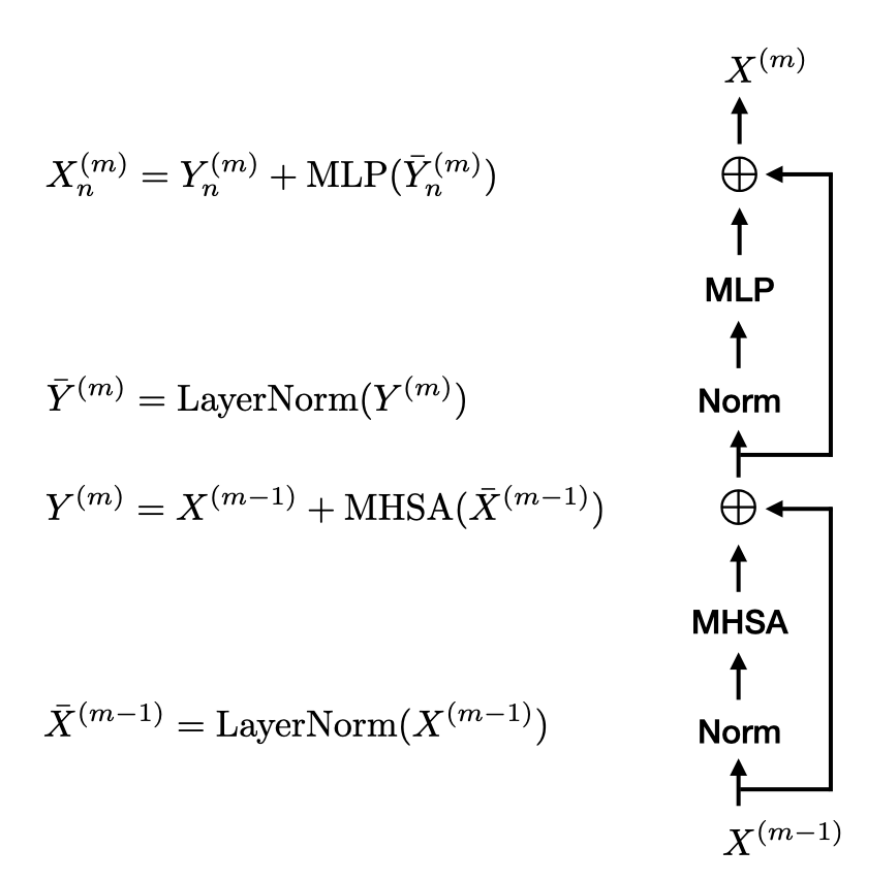
\includegraphics[width=0.6\textwidth]{models/preliminaries/imgs/transformer-block.png}
    \caption{Image taken from \cite{turnerIntroductionTransformers2024}, Transformer Block architecture.}
    \label{fig:transformer_block}
\end{figure}

\noindent In order to refer to the architecture,
that is Multi Headed Self-Attention with dimension $d \in \mathbb N$ and number of heads $H \in \mathbb N$,
whose weights are not fixed but subject to optimization, 
we write $\text{MSA}(d, H)$.

\noindent Given a number of heads $H \in \mathbb N$ typically the embedding dimension of each head is chosen as $\frac{d}{H}$.

\noindent Another key ingredient for Transformer models is layer normalization.

\begin{definition}[Layer Normalization]
    Let $\gamma \in \mathbb R$ and $\beta \in \mathbb R^d$. The operation given by

        $$\text{LN} : \mathbb R^d \to \mathbb R^d ~, ~~ 
        \text{LN}(x) = \gamma \bar{x} + \beta 
        \text{ where } \bar{x}_{ki} = \frac{1}{\sqrt{\text{var}(x_{k})}} (x_{ki} - \sum_{j=1}^d x_{kj})$$

    is called layer normalization.
\end{definition}

Typically Multi Headed Self-Attention is used in transformer blocks,
the architecture is outlined in figure \ref{fig:transformer_block}.
We describe this operation formally in the next definition.

\begin{definition}[Transformer Block] 
    \label{def:transformer_block}
    Let $d, H \in \mathbb N$ and $\Phi: \mathbb{R}^d \to \mathbb{R}^d$ be some mapping.
    The architecture 

        \begin{equation*}
            T(d, H, \Phi) = R \big( \Phi \circ \text{LN} \big) \circ R \big( \text{MSA}(d, H) \circ \text{LN} \big)
        \end{equation*}

    is called a Transformer Block.
\end{definition}

Typically the mapping $\Phi$ is some neural network, with only a few number of layers.
The tokens are processed individually by the mapping $\Phi$, so the sequence is treated as a batch.

\vspace{2mm}

Transformers operate on sequential data, 
so how to apply these models to images?
In their 2020 paper \textit{An image is worth 16 $\times$ 16 words: Transformers for image recognition at scale},
Dosovitskiy et al. \cite{dosovitskiyImageWorth16x162021} propose to partition image data $X \in \mathbb R^{C \times H \times W}$
into a sequence of patches, in order to bridge the gap between the two domains.
An image is partitioned into patches sized $P \times P$, for some $P \in \mathbb N$, 
these are flattened and embedded using a linear mapping to obtain a sequence $(x_k)_{k=1}^N \in S (R^{C \cdot P^2})$,
where $N = \frac{HW}{P^2}$. 
Let $w = \frac{W}{P}$, mathematically the partitioning can be described as follows 

    \begin{equation} \label{eq:vit_patch}
        \hat{x}_{k}( i_c P^2 + i_h P + i_w) = X \left( i_c, \left\lfloor \frac{k}{w} \right\rfloor + i_h, k \mod w + i_w \right) ~,
    \end{equation}

for $k = 1, ..., N$, $i_c = 1, ..., C$ and $i_h, i_w = 1, ..., P$.
The flattened patches are embedded to obtain the sequence of tokens $(x_k)_{k=1}^N$,
that is

    $$ x_k = E \hat{x}_k ~, $$

for some $E \in \mathbb R^{D \times C \cdot P^2}$.
We implicitly assume that $H \mod P = W \mod P = 0$, i.e. both the height and the width are devisable by the patch size $P$.
The approach is also visualized in figure \ref{fig:vit}.

\begin{figure}[h!]
    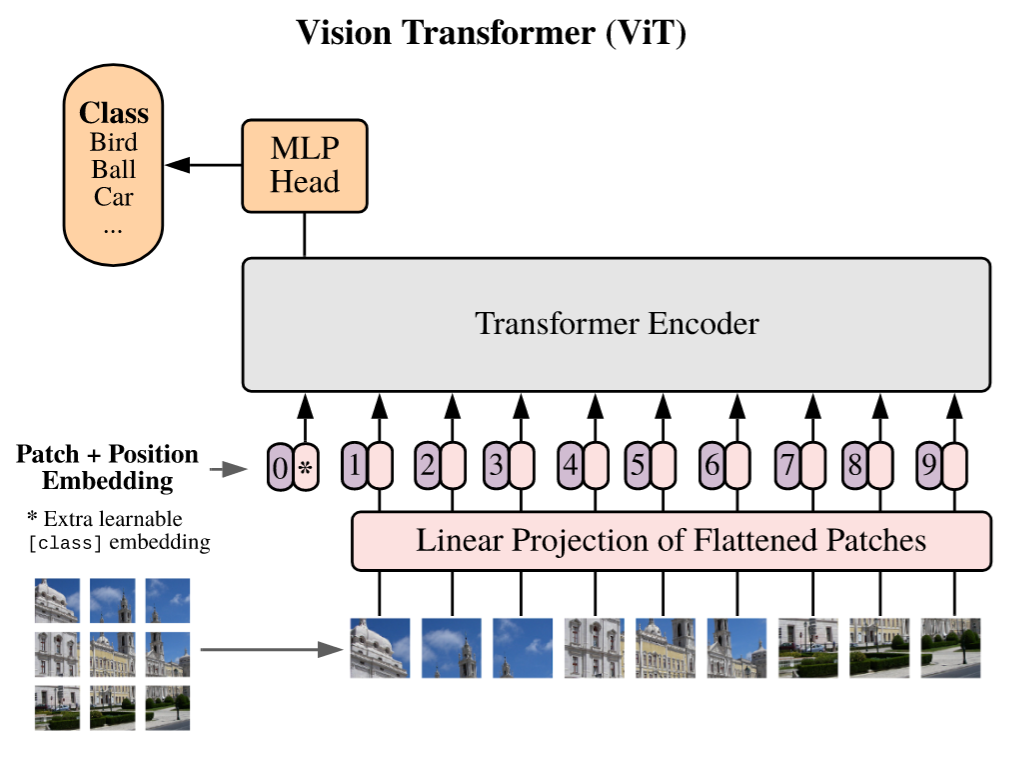
\includegraphics[width=0.6\textwidth]{models/preliminaries/imgs/vit.png}
    \caption{Image taken from \cite{dosovitskiyImageWorth16x162021}, Vision Transformer.}
    \label{fig:vit}
\end{figure}

Liu et al. \cite{liuSwinTransformerHierarchical2021} point out,
that unlike in language, where a word naturally offers itself as the atomic unit,
visual elements vary in scale,
making the fixed patch sizes unsuitable for tasks requiring predictions at pixel level,
as for example semantic segmentation. 
Simply treating each individual pixel as a token would solve the problem,
but at the same time introduce immense computational complexity.
For a full HD image of size $1920 \times 1080$ this leads to a sequence length of $2.0736 \cdot 10^{6}$.
Thus to reduce computational complexity,
but at the same time maintain a global receptive field, 
Liu et al. \cite{liuSwinTransformerHierarchical2021} propose Hierarchical Shifted Window Transformers (SWinT).

As before the image is partitioned into non-overlapping patches,
as described in equation (\ref{eq:vit_patch}), 
Liu et al. \cite{liuSwinTransformerHierarchical2021} opt for a patch size $P = 4$,
to obtain a sequence of tokens $(x_k)_{k=1}^N$.
The tokens are then partitioned into subsequences

    \begin{equation*} 
        \left(x_{k^{(1)}_l} \right)_{l=1}^{M^2}, ..., \left(x_{k^{(N')}_l} \right)_{l=1}^{M^2}
    \end{equation*}

where $N' = \frac{HW}{4^2 M^2}$.
The subsequences $(k_l^{(p)})_{l=1}^{M^2}$ are chosen so that neighboring patches form a super patch of size $M \times M$, 
for some $M \in \mathbb N$, formally that is

    \begin{equation} \label{eq:super_partitioning}
        k_l^{(p)} = \underbrace{M^2 \cdot \left \lfloor \frac{p}{\left( \frac{W}{4M} \right)}\right \rfloor}_\text{inter patch row}
        + \underbrace{M \cdot \left( p \mod \frac{W}{4M} \right)}_\text{inter patch column}
        + \underbrace{\left \lfloor \frac{l}{M}\right \rfloor \cdot \left( \frac{W}{4M} - 1 \right)}_\text{intra patch row}
        + \underbrace{l}_\text{intra patch column} ~,
    \end{equation}

for all $p = 1, ..., N'$ and $l = 1, ..., M^2$, 
we are enumerating the super patches from left to right, top to bottom, 
note that $\frac{W}{4P}$ returns the number of super patches along the horizontal axis.
Self-attention is then performed locally inside of each super patch

    \begin{equation} \label{eq:swin1}
        (y_{k^{(p)}_l})_{l=1}^{M^2} = \text{MSA}(Q, K, V) \left( (x_{k^{(p)}_l})_{l=1}^{M^2} \right) ~,
    \end{equation}

for $p = 1, ..., N'$, for some $Q, K, V \in \mathbb R^{H \times \frac{d}{H} \times d}$.

If equation (\ref{eq:swin1}) would be used repeatedly to update features,
information is restricted to flow only inside individual super patches. 
To establish information flow amongst super patches, 
Liu et al. \cite{liuSwinTransformerHierarchical2021} introduce the shifted window mechanism.
Consecutive operations of self-attention use different partitionings of the sequence $(x_k)_{k=1}^N$.
We consider the partitioning described in equation (\ref{eq:swin_partitioning}) as the unshifted variant,
for the shifted partitioning the borders of the patches are moved down and to the right by $s = \left \lfloor \frac{P}{2} \right \rfloor$ units.
In order to achieve the shift, while keeping the same partitioning, a cyclic shift is applied to the feature map,
it is visualized in figure \ref{fig:cyclic_shift}. Formally, this can be described by processing an auxilliary feature map $X' \in \mathbb R^{C \times H \times W}$,
defined by

    \begin{equation} \label{eq:cyclic_shift}
        X'(c, i, j) = X \big(c, (i + s) \mod H , (j + s) \mod W \big) ~,
    \end{equation}

for $c = 1, ..., C$, $i = 1, ..., H$ and $j = 1, ..., W$.
Instead also padding techniques could be applied,
but Liu et al. \cite{liuSwinTransformerHierarchical2021} report achieving better results, 
whilst saving computational complexity by employing the cyclic shift.

\begin{figure}[h!]
    \begin{center}
        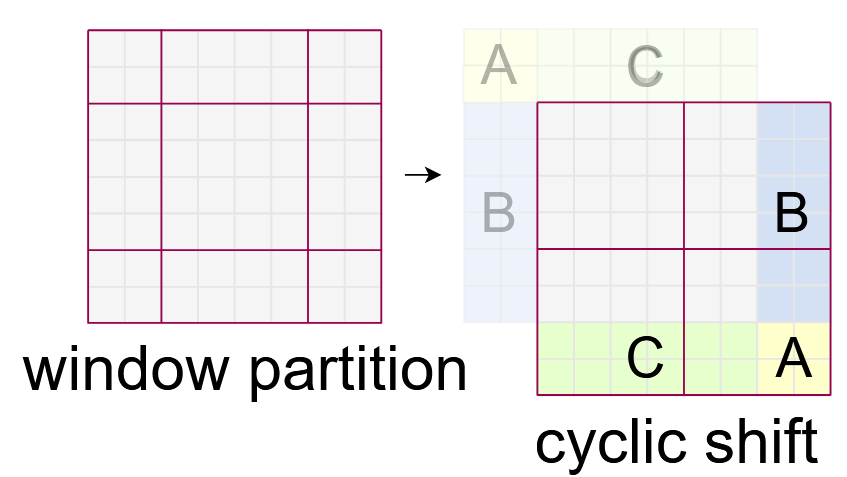
\includegraphics[width=0.6\textwidth]{models/preliminaries/imgs/cyclic-shift.png}
    \end{center}
    \caption{Image taken from \cite{liuSwinTransformerHierarchical2021}, visualizing the cyclic shift.
        Here the pixels in the image are rearranged, and then the unshifted partitioning is used, to obtain the cyclic shift.}
    \label{fig:cyclic_shift}
\end{figure}

\begin{definition}[Cyclic shift]
    \label{def:partitioning}
    We denote the function implementing equation (\ref{eq:cyclic_shift}) by
    \begin{equation*}
        \text{CS}: \mathbb R^{C \times H \times W} \to \mathbb R^{C \times H \times W} ~, ~~
        \text{CS}(X) = X' ~.
    \end{equation*}
\end{definition}

To enable a global receptive field, 
Liu et al. \cite{liuSwinTransformerHierarchical2021} propose to merge neighboring patches, 
after the inputs are processed by a certain number of SWin TransformerBlocks.
To this end patches $P_1, ..., P_4 \in \mathbb R^{C \times P \times P}$,
inside a neighborhood of size $2 \times 2$ are stacked along the channel dimension,
to form a super patch $\hat{P} = [P_1, ..., P_4] \in \mathbb R^{4 \cdot C \times P \times P}$.
To fuse the features a convolutional layer is applied, 
halving the channel dimension of the super patch

    \begin{equation*}
        P = C(4 \cdot C, 2 \cdot C, \text{kernel-size}=3, \text{padding}=1)(\hat{P}) ~.
    \end{equation*}

This process is repeated until the entire feature map is of size $P \times P$.
We implicitly assume that $H = 2^{n_1} P$ and $W = 2^{n_2} P$ for some $n_1, n_2 \in \mathbb N$.
The overall architecture of the SWin Transformer is shown in figure \ref{fig:swin}.

\begin{figure}[h!]
    \begin{center}
        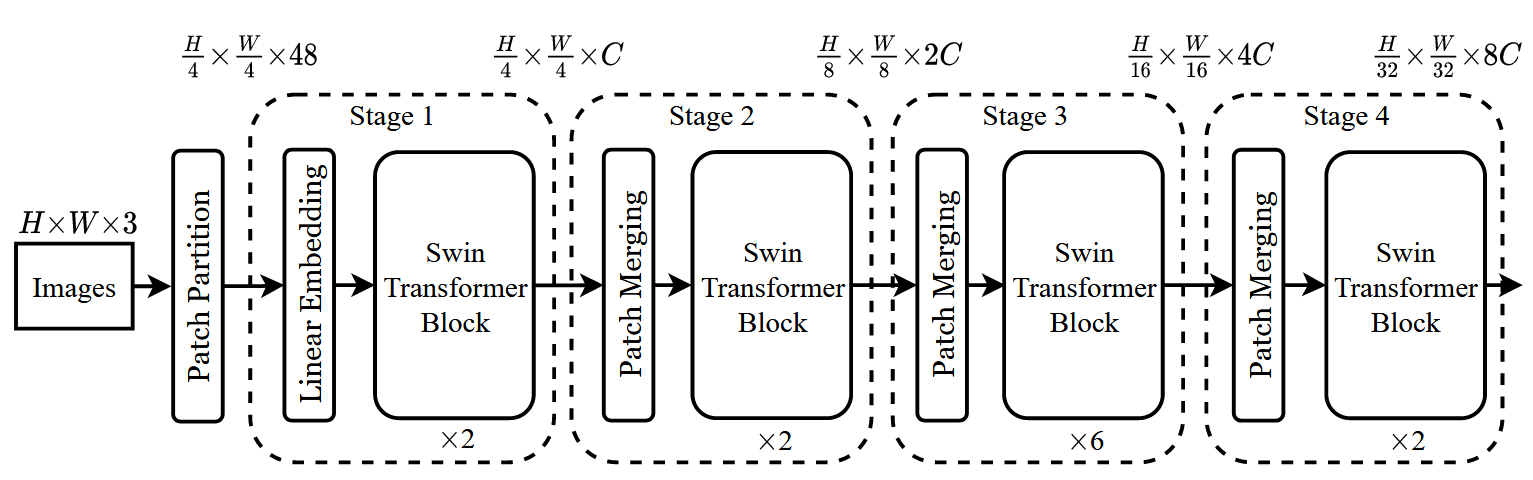
\includegraphics[width=0.6\textwidth]{models/preliminaries/imgs/swin.png}
    \end{center}
    \caption{Image taken from \cite{liuSwinTransformerHierarchical2021}, SWin Transformer.}
    \label{fig:swin}
\end{figure}

\begin{definition}[Shifted window Transformer Block]
    Let $d, H \in \mathbb N$ and $\Phi_1, \Phi_2: \mathbb R^d \to \mathbb R^{d}$.
    The architecture given by

        \begin{equation*}
            \text{SWinT}(d, H, \Phi_1, \Phi_2) = \text{T}(d, H, \Phi_2) \circ \text{CS}\circ \text{T}(d, H, \Phi_1) ~.
        \end{equation*}

    is called Shifted Window Transformer Block.
\end{definition}

Chen et al. \cite{chenHATHybridAttention2024} introduce overlapping Cross Attention (OCA),
a modification of SWin Transformers.
Whilst in equation (\ref{eq:super_partitioning}) the patches are constructed to partition the feature map,
OCA establishes cross patch connections,
by constructing the patches so that they overlap.
Formally, let $\gamma \in (0, 1)$ be the factor of overlap and $p = 1, ..., N$ index the patches.
Let $M_o = \lfloor (1 + 2\gamma)M \rfloor$, the subsequences associated to patch $p$ is given by

\begin{equation} \label{eq:oca_partitioning}
    k_l^{(p)} = \underbrace{M^2 \cdot \left \lfloor \frac{p}{\left( \frac{W}{4M} \right)}\right \rfloor}_\text{inter patch row}
        + \underbrace{M \cdot \left( p \mod \frac{W}{4M} \right)}_\text{inter patch column}
        + \underbrace{\left \lfloor \frac{l}{M_o}\right \rfloor \cdot \left( \frac{W}{4M_o} - 1 \right)}_\text{intra patch row}
        + \underbrace{l - \gamma M}_\text{intra patch column} 
        + \underbrace{\gamma M}_\text{padding} ~,
\end{equation}

for $l = 1, ..., M_o^2$, note padding was added and only the terms responsible for intra patch indexing were manipulated,
this way the overlap is guaranteed.

\noindent Super patches sharing an edge have an overlap of $\left \lfloor \gamma M \right \rfloor M$ pixels,
whereas super patches sharing only a corner have an overlap of $ \left \lfloor \gamma M \right \rfloor^2$ pixels.
For query, key and value matrices $Q, K, V \in \mathbb R^{d', d}$, 
for a patch $p = 1, ..., P$, 
the attention scores are computed in the following way

    \begin{equation} \label{eq:oca1}
        A_{ij} = \frac{\text{exp}({x_{i}^{(p)}}^T K^T Q x_{j}^{(p)})}{\sum_{k = 1}^n \text{exp}({x_{k}^{(p)}}^T K^T Q x_{j}^{(p)})} ~,
    \end{equation}

for $i = 0, ..., M_o$
and $j = \left \lfloor \gamma M \right \rfloor, ..., M + \left \lfloor \delta M \right \rfloor$.
The outputs are then computed for all $j = \left \lfloor \gamma M \right \rfloor, ..., M + \left \lfloor \gamma M \right \rfloor$ by 

    \begin{equation} \label{eq:oca2}
        y_{j} = \sum_{i=1}^n A_{ij} V x_{i} ~.
    \end{equation}

Thereby every token is updated exactly once, 
while capturing information from tokens belonging to other partitions.
Note that equation (\ref{eq:sa1}) and (\ref{eq:oca1})
differ only by the indices attained by $j$,
leading to the queries only coming from the part of the super patch,
which is not shared by others.
The operation is visualized in figure \ref{fig:ocab}.

\begin{figure}[h!]
    \begin{center}
        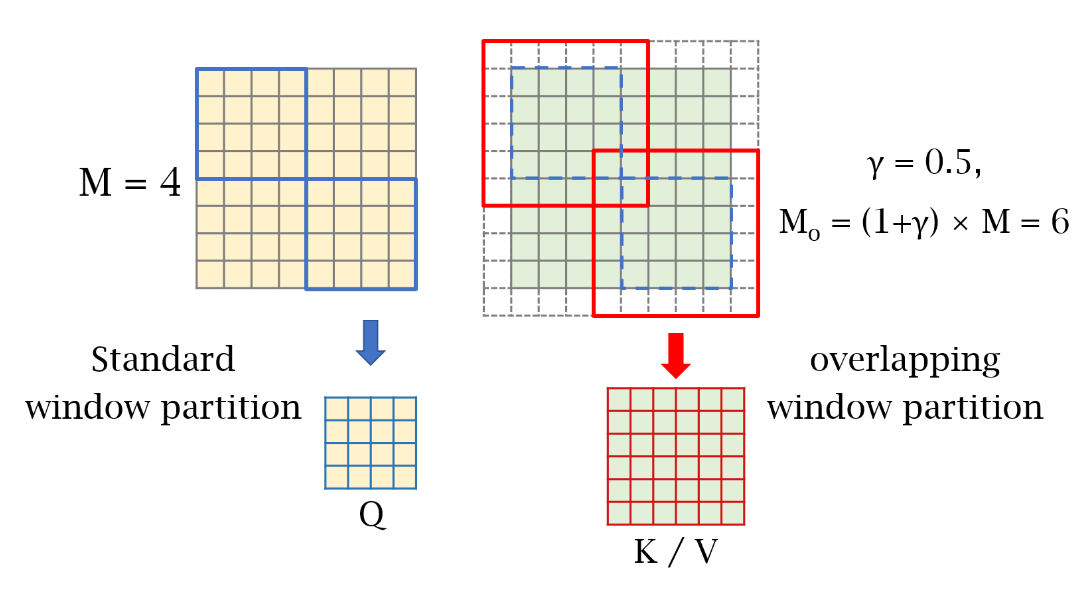
\includegraphics[width=0.6\textwidth]{models/preliminaries/imgs/ocab.png}
    \end{center}
    \caption{Image taken from \cite{chenHATHybridAttention2024}, Overlapping Cross-Attention Block.}
    \label{fig:ocab}
\end{figure}

We conclude this chapter by introducing definitions for
overlapping cross-attention, multi headed overlapping cross-attention and overlapping cross-attention block
analogously to the definitions \ref{def:partitioning}, \ref{def:sa}, \ref{def:msa} and \ref{def:transformer_block}.

\begin{definition}[Overlapping Cross-Attention]
    \label{def:oca}
    Let $Q, K, V \in \mathbb R^{d', d}$.
    The operation described in equations (\ref{eq:oca1}), (\ref{eq:oca2}), that is

        $$ \text{OCA}: S(\mathbb R^{d}) \to S(\mathbb R^{d}) ~, 
        ~~ \text{OCA} (Q, K, V) \big( (x_k)_{k=1}^N \big) = (y_k)_{k=1}^N ~, $$

    \noindent is called overlapping cross-attention.
\end{definition}

Analogously to standard self-attention, 
we also introduce multi headed overlapping cross-attention.

\begin{definition}[Multi Headed Overlapping Cross-Attention]
    \label{def:moca}
    Let $Q_h, K_h, V_h \in \mathbb R^{d', d}$ for $h= 1,..., H$ and let $Q = (Q_1, ..., Q_H), K = (K_1, ..., K_H), V = (V_1, ..., V_H)$.
    The operation
        $$ \text{MOCA}(Q, K, V) \left((x_{k})_{k=1}^n \right) = \big[\text{OCA}(Q_1, K_1, V_1)\left((x_{k})_{k=1}^n \right), ..., \text{OCA}(Q_H, K_H, V_H)\left((x_{k})_{k=1}^n \right) \big] ~, $$
    \noindent is called multi headed overlapping cross-attention.
\end{definition}

\begin{definition}[Overlapping Cross-Attention Block]
    \label{def:oca_block}
    Let $\delta \in (0, 1)$, $d, H \in \mathbb N$ and $\Phi: \mathbb{R}^d \to \mathbb{R}^d$ be some mapping.
    The architecture 

        \begin{equation*}
            \text{OCAB}(d, H, \Phi) = R \big( \Phi \circ \text{LN} \big) \circ R \big( \text{MOCA}(d, H) \circ \text{LN} \big) \circ P(\delta)
        \end{equation*}

    \noindent is called a Overlapping Cross-Attention Block.
\end{definition}